\section{Theoretical Analysis}
\label{sec:analysis}

In this section, the circuit shown in Figure~\ref{fig:rc} is analysed
theoretically.

\subsection{Nodal Analysis}

The first step we took was analyzing the circuit for t<0 and by applying Kirchhoff's Current and voltage Laws we determined the currents in branches and voltage in nodes respectively. This are the equations used by us.

In node 1 we also considered:
\begin{equation}
	V_1 = V_s | V_4 = 0
\end{equation}


Using the equations above, we get the following matrix equation:

\begin{gather}
	\begin{bmatrix}
		G_1 & -(G_1 + G_2 + G_3) & G_2 & 0 & G_3 & 0 & 0 & 0 \\ 
		0 & K_b + G_2 & -G_2 & 0 & -K_b & 0 & 0 & 0 \\
		0 & K_b & 0 & 0 & -(K_b + G_5) & G_5 & 0 & 0 \\ 
		0 & 0 & 0 & G_6 & 0 & 0 & -(G_6 + G_7) & G_7 \\
		1 & 0 & 0 & -1 & 0 & 0 & 0 & 0 \\
		0 & 0 & 0 & -K_bG_6 & -1 & 0 & K_bG_6 & 1 \\
		0 & G_3 & 0 & G_4 & -(G_3 + G_4 + G_5) & G_5 & G_7 & -G_7
	\end{bmatrix}
	\begin{bmatrix} V_1 \\ V_2 \\ V_3 \\ V_4 \\ V_6 \\ V_7 \\ V_8 \end{bmatrix}
	=
	\begin{bmatrix} 0 \\ 0 \\ 0 \\ 0 \\ V_s \\ 0 \\ 0 \end{bmatrix}
\end{gather}

Using octave we obtain the following table:
\begin{table}[!h]
	\centering
	\begin{tabular}{|l|r|}
		\hline    
		{\bf Name} & {\bf Value [mA]} \\ \hline
		§R1 & 1.04309563061e+03 \\ \hline
§R2 & 2.01744623407e+03 \\ \hline
§R3 & 3.13691375104e+03 \\ \hline
§R4 & 4.15429988186e+03 \\ \hline
§R5 & 3.07915362723e+03 \\ \hline
§R6 & 2.02592738504e+03 \\ \hline
§R7 & 1.04226655522e+03 \\ \hline
§H1 & 8.25247516035e+03 \\ \hline
£G1 & 7.31630468385e-03 \\ \hline
Va & 5.23936486299e+00 \\ \hline
@Id & 1.03899051042e-03 \\ \hline


	\end{tabular}
	\caption{Constants provided by Python. A variable preceded by @ is of type {\em current}
		and expressed in Ampere;a variable preceded by § is of type {\it resistence} and expressed in
		Ohms;a variable preceded by £ is of type {\it conductance} and expressed in
		Siemens; other variables are of type {\it voltage} and expressed in
		Volt.}
	\label{tab:op}
\end{table}

Using Ohms law, we can calculate the current flowing through each resistor, which are represented in the following table:
 \begin{table}[!h]
 	\centering
 	\begin{tabular}{|l|r|}
 		\hline    
 		{\bf Name} & {\bf Value [mA]} \\ \hline
 		§R1 & 1.04309563061e+03 \\ \hline
§R2 & 2.01744623407e+03 \\ \hline
§R3 & 3.13691375104e+03 \\ \hline
§R4 & 4.15429988186e+03 \\ \hline
§R5 & 3.07915362723e+03 \\ \hline
§R6 & 2.02592738504e+03 \\ \hline
§R7 & 1.04226655522e+03 \\ \hline
§H1 & 8.25247516035e+03 \\ \hline
£G1 & 7.31630468385e-03 \\ \hline
Va & 5.23936486299e+00 \\ \hline
@Id & 1.03899051042e-03 \\ \hline


 	\end{tabular}
 	\caption{Constants provided by Python. A variable preceded by @ is of type {\em current}
 		and expressed in Ampere;a variable preceded by § is of type {\it resistence} and expressed in
 		Ohms;a variable preceded by £ is of type {\it conductance} and expressed in
 		Siemens; other variables are of type {\it voltage} and expressed in
 		Volt.}
 	\label{tab:op}
 \end{table}
 

\subsection{Equivalent Resistance}
A set of equations were used, bearing in mind that the Thévenin Theorem was applied. By applying this theorem, all the independent tension sources were considered null, to study the influence of the condenser in the circuit, in order to obtain the circuit´s equivalent resistance in the perspective of the circuit extremities. We assumed that the tension $V_s = 0V$ and there was a passage from a constant value to null value, which was the result of the passage of a non-null current passing through the condenser. Also, since the voltage source interior resistance was null, it's the equivalent to cause a short-circuit to that source.

The Kirchhoff's Laws can also be applied here, leading to the same equations used in the section before. The rest of the equations can be obtained using the following equation:
\begin{equation}
	V_x = V_6 - V_8
\end{equation}

With former equations, we can form the matrix equation used bellow:
\begin{gather}
	\begin{bmatrix}
		G_1 & -(G_1 + G_2 + G_3) & G_2 & 0 & G_3 & 0 & 0 & 0 \\ 
		0 & K_b + G_2 & -G_2 & 0 & -K_b & 0 & 0 & 0 \\
		0 & 0 & 0 & 0 & 0 & 1 & 0 & -1 \\ 
		0 & 0 & 0 & G_6 & 0 & 0 & -(G_6 + G_7) & G_7 \\
		1 & 0 & 0 & -1 & 0 & 0 & 0 & 0 \\
		0 & 0 & 0 & -K_dG_6 & -1 & 0 & K_dG_6 & 1 \\
		-G_1 & G_1 & 0 & -(G_4 + G_6) & G_4 & 0 & G_7 & 0
	\end{bmatrix}
	\begin{bmatrix} V_1 \\ V_2 \\ V_3 \\ V_4 \\ V_6 \\ V_7 \\ V_8 
	\end{bmatrix}
	=
	\begin{bmatrix} 0 \\ 0 \\ V_x \\ 0 \\ 0 \\ 0 \\ 0 
	\end{bmatrix}
\end{gather}

Using octave we get the following data:
\begin{table}[!h]
	\centering
	\begin{tabular}{|l|r|}
		\hline    
		{\bf Name} & {\bf Value [mA]} \\ \hline
		§R1 & 1.04309563061e+03 \\ \hline
§R2 & 2.01744623407e+03 \\ \hline
§R3 & 3.13691375104e+03 \\ \hline
§R4 & 4.15429988186e+03 \\ \hline
§R5 & 3.07915362723e+03 \\ \hline
§R6 & 2.02592738504e+03 \\ \hline
§R7 & 1.04226655522e+03 \\ \hline
§H1 & 8.25247516035e+03 \\ \hline
£G1 & 7.31630468385e-03 \\ \hline
Va & 5.23936486299e+00 \\ \hline
@Id & 1.03899051042e-03 \\ \hline


	\end{tabular}
	\caption{Constants provided by Python. A variable preceded by @ is of type {\em current}
		and expressed in Ampere;a variable preceded by § is of type {\it resistence} and expressed in
		Ohms;a variable preceded by £ is of type {\it conductance} and expressed in
		Siemens; other variables are of type {\it voltage} and expressed in
		Volt.}
	\label{tab:op}
\end{table}


\subsection{Natural Solution}

In this section we will start by analyzing the natural solution , where t varies from 0 to 20 ms, by using the equivalent resistance we calculated before.

Assim that $V_0 = V_x$, the natural solution of the capacitor is  
\begin{equation}
	V_6n(t) = V_xe^{-(t)/CR_eq}
\end{equation}

We can now plot the graph of the solution for t raging from 0 to 20 ms:

\begin{figure}[h] \centering
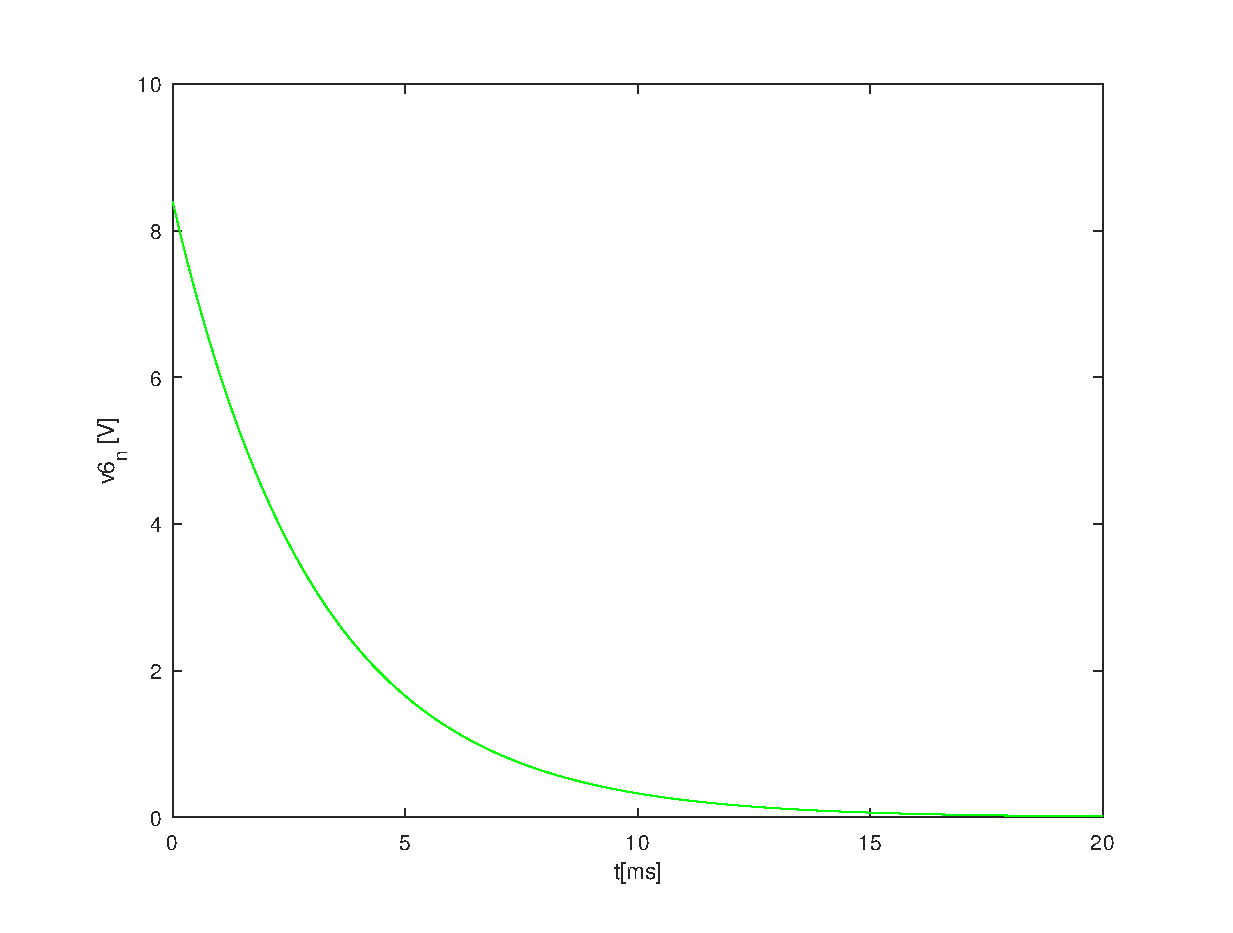
\includegraphics[width=0.6\linewidth]{natural.eps}
\caption{.}
\label{fig:rc1}
\end{figure}
	
\subsection{Forced Solution}

The nodal analysis of this circuit, is done with the tension phasor being equal to 1 and the condenser has an impedance of$\frac{1}{iwc}$.
After this, we make the same analysis, which can be represented by the following matrix:
\begin{gather}
	\begin{bmatrix}
		G_1 & -(G_1 + G_2 + G_3) & G_2 & 0 & G_3 & 0 & 0 & 0 \\ 
		0 & K_b + G_2 & -G_2 & 0 & -K_b & 0 & 0 & 0 \\
		0 & K_b & 0 & 0 & -(K_b + G_5) & Y_c + G_7 & 0 & -Y_c \\ 
		0 & 0 & 0 & G_6 & 0 & 0 & -(G_6 + G_7) & G_7 \\
		1 & 0 & 0 & -1 & 0 & 0 & 0 & 0 \\
		0 & 0 & 0 & -K_dG_6 & -1 & 0 & K_dG_6 & 1 \\
		0 & G_3 & 0 & -G_4 & -(G_3 + G_4 + G_5) & G_5 + Y_c & G_7 & -(G_7 + Y_c)
	\end{bmatrix}
	\begin{bmatrix} V_1 \\ V_2 \\ V_3 \\ V_4 \\ V_6 \\ V_7 \\ V_8 
	\end{bmatrix}
	=
	\begin{bmatrix} 0 \\ 0 \\ 0 \\ 0 \\ 1 \\ 0 \\ 0 
	\end{bmatrix}
\end{gather}

\begin{table}[!h]
	\centering
	\begin{tabular}{|l|r|}
		\hline    
		{\bf Name} & {\bf Value [mA]} \\ \hline
		§R1 & 1.04309563061e+03 \\ \hline
§R2 & 2.01744623407e+03 \\ \hline
§R3 & 3.13691375104e+03 \\ \hline
§R4 & 4.15429988186e+03 \\ \hline
§R5 & 3.07915362723e+03 \\ \hline
§R6 & 2.02592738504e+03 \\ \hline
§R7 & 1.04226655522e+03 \\ \hline
§H1 & 8.25247516035e+03 \\ \hline
£G1 & 7.31630468385e-03 \\ \hline
Va & 5.23936486299e+00 \\ \hline
@Id & 1.03899051042e-03 \\ \hline


	\end{tabular}
	\caption{Constants provided by Python. A variable preceded by @ is of type {\em current}
		and expressed in Ampere;a variable preceded by § is of type {\it resistence} and expressed in
		Ohms;a variable preceded by £ is of type {\it conductance} and expressed in
		Siemens; other variables are of type {\it voltage} and expressed in
		Volt.}
	\label{tab:op}
\end{table}

\subsection{Total Solution}
We can obtain $v_6t(t)$ (the total solution), by superimposing the natural(section 2.2.) and forced solutions (2.3) obtained before. Since we determined the function of the natural solution in section 2.2 we will now determine the forced solution.

The complex equation of the phasor can be written as:
\begin{equation}
	v_6f(t) = V_6sen(\omega t + \varphi_s)
\end{equation}

In the equation above, $\omega = 2\pi f = 2000\pi$ and $\varPhi$ is the argument of 

By superimposing the equations of both the natural and forced solutions, we obtain this equation:

\begin{equation}
	v_6(t) = v_6n(t) + V_6f(t) = V_6sen(\omega t + \varphi_s) + V_xe^{-(1)/R_sC}
\end{equation}

By plotting this function, for t in range of -5 to 20 ms, we get the graph below:


\begin{figure}[h] \centering
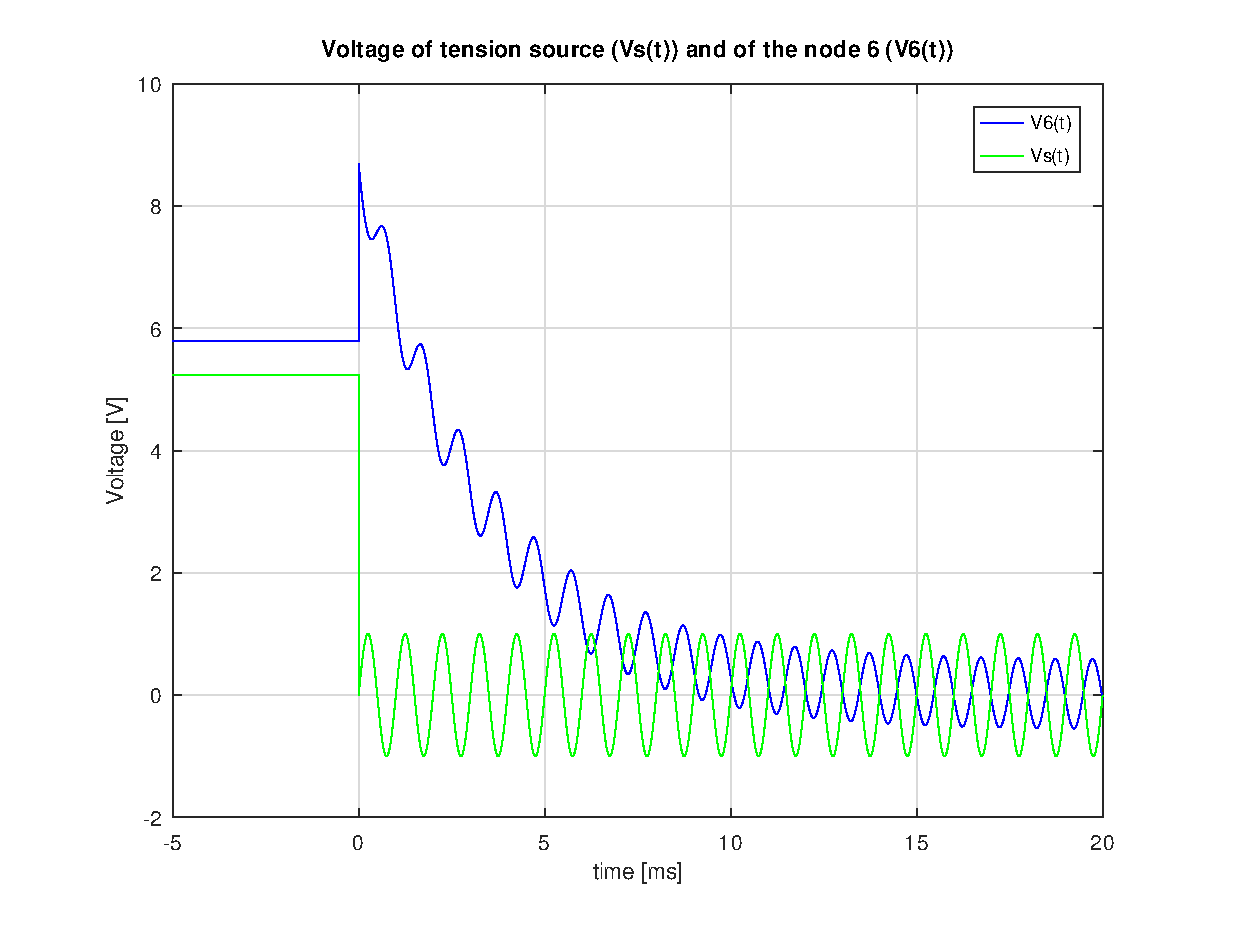
\includegraphics[width=0.6\linewidth]{forced_solution.eps}
\caption{.}
\label{fig:rc2}
\end{figure}

\subsection{Frequency Response}

Lastly, we will analyze the frequency response of each phasor, by applying the same method used in section 2.4, with the exception that $Y_c$ wil remain as a variable ($Y_c(f) = j2\pi fC$).

Considering:
\begin{equation}
	V_c(t) = V_6(t) - V_8(t)
\end{equation} 

Next we can plot the graphs of $V_c(t)$ and $V_6(t)$, as functions of f in range of $10^(-1)$ to $10^(6)$ Hz, which will be defined as logarithmic scales.

The magnitude plot has values in dB, which respect the following equation:
\begin{equation}
	V_dB = 20\log_10(V)
\end{equation}

The graphics of the plotted functions $v_c(f)$ and $v_6(f)$:


\graphicspath{ {./images/} }

a

\includegraphics{universe}



\graphicspath{ {./images/} }

a

\includegraphics{universe}
